\question
В городе N очень хотят построить метро. Матрица смежности взвешенного графа, представляющего схему связей между предполагаемыми станциями, указана ниже.

\begin{minipage}[h]{0.45\linewidth}
\center{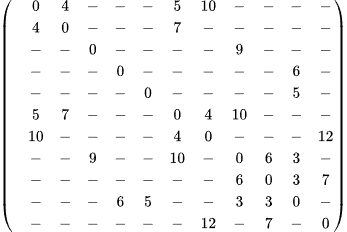
\includegraphics[width=0.7\textwidth]{pic/72.png} }
\end{minipage}

Постройте граф по данной матрице, укажите:
\begin{enumerate}
\item Как следует построить метро, чтобы каждый пункт был доступен из другого, но суммарное расстояние между всеми станциями было минимальным. Покажите на графе.
\item Сколько переездов между станциями (граф п.1) необходимо добавить, чтобы можно было объехать все станции, посещая каждую ровно по одному разу?
\item Сколько ребер необходимо добавить в граф из п.1, чтобы существовал путь, проходящий через все переезды по одному разу?
\end{enumerate}

---------------

Автор -- Елизавета Котельникова
